\documentclass[12pt, letterpaper]{article}

\usepackage[margin=1in]{geometry}

\usepackage[parfill]{parskip}

\usepackage{scrextend}

\usepackage{amssymb, amsmath, mathtools, bbm, cancel}

\usepackage[linesnumbered,lined,boxed]{algorithm2e} % algorithm environment
\usepackage{xpatch} % forces algo enviro to fit in line width
	\xpretocmd{\algorithm}{\hsize=\linewidth}{}{}

\allowdisplaybreaks

\usepackage{fancyhdr, color, pgfplots}

\usepgfplotslibrary{fillbetween}
\usetikzlibrary{patterns}
\pgfplotsset{compat=1.12}

\definecolor{myorange}{HTML}{EF8B21} % custom orange
\definecolor{mygreen}{HTML}{6F9A48} % custom green
\definecolor{myblue}{HTML}{008BA9} % custom blue

\renewcommand{\thefootnote}{\roman{footnote}} % makes footnotes roman numerals

\begin{document}
\begin{titlepage}
	\begin{center}
		\vspace*{.5in}
        
		\Huge
		\textsc{Final Project Written Summary}
        
		\Large
		\textsc{Cryptocurrency Statistical Arbitrage Strategy}
        
		\vfill
		
		\normalsize
		Rushabh \textsc{Nahar} \\
		Aishwarya \textsc{Sinh} \\
		Sanat \textsc{Shah} \\
		Casey \textsc{Tirshfield}
        
		\vfill
		
		IEOR E4729 Model Based Trading \\
		Columbia University \\
		\today
		
		\vspace*{.5in}
        
	\end{center}
\end{titlepage}

\begin{abstract}
\noindent For our final project we have designed and implemented (in simulation) a cointegration based pairs trading strategy. Traditionally, this type of strategy has been employed only for stocks and exchange traded funds. In our project, however, we apply the strategy to the top 100 cryptocurrencies by market capitalization. The generally cointegrated nature of cryptocurrencies, and their burgeoning popularity, make them ideal candidates for a successful implementation of this method.
\end{abstract}

\section{Motivation}
In delineating the scope of this project we made three major decisions. Our first decision was to implement a pairs trading strategy. Our second decision was to use this strategy on cryptocurrencies. And our final decision was to use a cointegration approach.

We decided to implement a pairs trading strategy because it is a proven method that has been tried and tested in the industry since the 80's. Moreover, it is market neutral and has a built in hedge---it matches a long position with a short position. This built in hedge lends itself to reduced net drawdowns---losses from a losing position are tempered by the gains from a winning position.

While pairs trading has historically been used on stocks and exchange traded funds there are very few papers discussing its success with cryptocurrencies. Since cryptocurrencies are becoming not only more ubiquitous, but also more widely accepted, we decided to explore this.

Finally, having decided to apply pairs trading to cryptocurrencies, applying the cointegration method was a natural progression. Cryptocurrencies largely move together in the markets meaning that they are prime candidates for cointigration.

\section{Assumptions}
\begin{enumerate}
	\item We assume that short selling is allowed. Currently, we are not allowed to shortsell in the cryptocurrency market. But our assumption is reasonable, since the expected introduction of futures contract for cryptocurrencies will allow us to short-sell. 
	\item Transaction cost is kept at 50 basis points. Generally, transaction costs in the Poloniex exchange is 0-25 basis points. However, we also need to consider the network fees and wallet fees. We discuss this further in section 3.
	\item At any point, we trade 10\% of the capital at hand. However, this assumes that our target pool of investors are more risk averse. 
	\item We set the p-value threshold at 0.5\%. We compare the p-value given by the algorithm to this threshold in order to test the null hypothesis for cointegration test.
\end{enumerate}

\section{Transaction Cost Analysis}
There are three types of transaction fees when dealing with cryptocurrencies:

\begin{enumerate}
	\item Exchange fees or commission: This is the commission paid to complete a buy or sell order. Generally a fixed-fee format but it depends on the crypto exchange. There is a model known as Market-Taker which exists within the crypto exchanges, where a variable fee based on amount of trading is charged.
	\item Network fees: This is the transaction fees paid to crypto miners. Miners are responsible for verifying and validating transactions that are supposed to be added to the blockchain. They ensure that tokens are not spent twice and the transaction is indeed valid. Miners set their own price.  The lower the price, the more time it will take for the miner to validate the transaction.
	\item Wallet fees: These are fees we pay in order to be able to store cryptos in our wallet.
\end{enumerate}

Since cryptocurrencies have such minimal transation costs, opening up two positions for a pairs trading strategy carries minimal cost and has the simultaneous benefit of hedging risk.

\section{Methodology}
	\subsection{Algorithm}
	\begin{enumerate}
		\item Find cointegrated pairs from the top 100 cryptocurrencies by market capitalization
		\item Perform an Engle-Granger two-step procedure on these pairs \begin{enumerate}
				\item[i.] Run an ordinary least squares regression in order to find the cointegration residual
				\item[ii.] Perform an Augmented Dickey-Fuller test on the following regression model: 
					\begin{equation*}
						\Delta y_t= \alpha + \delta y_{t-1}+\sum_{i=1}^{h}\Delta\beta_i y_{t-i}+\epsilon_t
					\end{equation*}
			\end{enumerate}
		\item Compare the output to the Dickey-Fuller test statistic: $$DF=\frac{\hat{\delta}}{\sqrt{\mathrm{Var}\left[\hat{\delta}\right]}}$$
		\item If the test statistic is smaller that the critical value (we assume the threshold p-value), the hypothesis is rejected. If the null is rejected, this would imply that there is no information gain from the inclusion of $y_{t-1}$ into the prediction of the variable $y_t$. This means that the series is stationary and no further data transformation is required. Expressing this mathematically, let $\xi$ be the critical value and $I(x)$ for $x\geq0$ be the order of integration.
			\begin{align*}
				H_0:& \quad DF=\xi\sim I(1) \quad\mathrm{not cointegrated} \\
				H_1:& \quad DF<\xi\sim I(0) \quad\mathrm{cointegrated}
			\end{align*}
	\end{enumerate}
	\subsection{Trading Strategy}
	We trade using the following rules:
	\begin{enumerate}
		\item If z-score is less than lower threshold, we long one unit of currency two and short beta units of currency one
		\item If z-score is greater than upper threshold, we short one unit of currency two and long beta units of currency one
		\item If the spread is narrow, we close our positions
	\end{enumerate}

	We rebalance our positions using the following rules:
	\begin{enumerate}
		\item If processes are cointegrated and the beta has changed, then we rebalance positions in both currencies using the new beta
		\item If processes are cointegrated and beta has not changes, then no rebalancing is required.
		\item If processes are not cointegrated anymore, we close all positions
	\end{enumerate}
	
\newpage
\section{Results}
This graph shows the time series plot of the data. The process is evidently co-integrated.
\begin{center}
	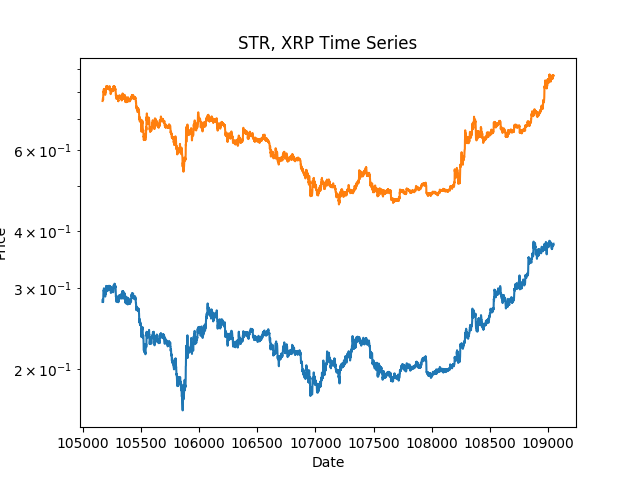
\includegraphics[scale=.5]{time_series_z2.png}
\end{center}
This is the plot for normalized spread. The threshold-levels of the z-score have been set to 2 standard deviations and whenever the spread crosses this level, trade signal is activated. When the spread is 0.5 standard deviations away we close all positions.
\begin{center}
	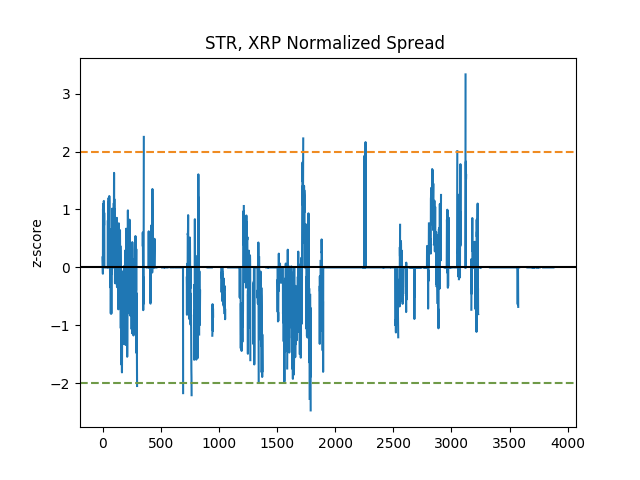
\includegraphics[scale=.5]{spread_z2.png}
\end{center}
This is the profit and loss plot for our crypto pair stellar and monero. We see a sudden spike in the PnL towards the end since the spread spikes above 3 standard deviations but then reverts back. Our strategy is able to exploit this statistical arbitrage and book a profit of about 9.5 percent for the trading period.
\begin{center}
	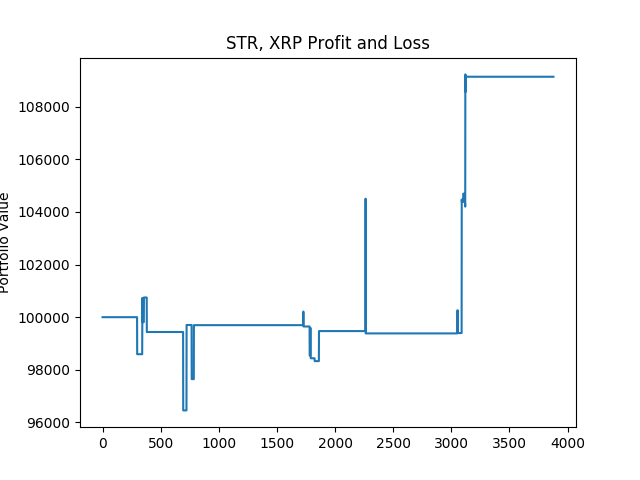
\includegraphics[scale=.5]{p&l_z2.png}
\end{center}
These are the portfolio positions during the trading period. We can compare this plot with the Normalized spread plot to confirm we hold positions only when the threshold is surpassed.
\begin{center}
	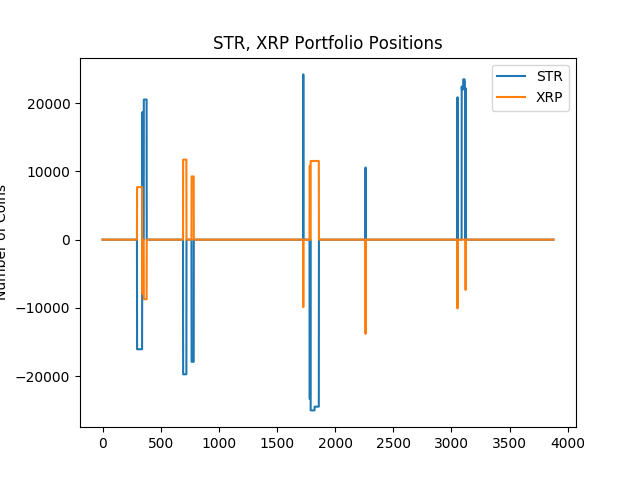
\includegraphics[scale=.5]{portfolio_z2.png}
\end{center}
	
\section{Conclusion and Challenges}

In completing this project, we recognized a few potential challenges which we attributed to either cryptocurrencies or pairs trading. For cryptocurrencies we found the following issues:
\begin{enumerate}
	\item The first cryptocurrency was created in 2008 and it was not until 2017 that the number of different cryptocurrencies exceeded 1000. Consequently, there is very little historical data from which we can draw. To add to this problem, many cryptocurrencies do not survive so the turnover in the market is huge.
	\item Another issue with cryptocurrencies is that of security. Since they only exist in the digital world they are susceptible to hacking. 
\end{enumerate}
For pairs trading we found the following issues:
\begin{enumerate}
	\item Due to high volatility in cryptocurrency markets, there is a risk that at execution the order will not be captured at the optimal price.
	\item Since in pairs trading we take both a long and short position, two times the standard commission must be paid.
\end{enumerate}
In conclusion, our pairs trading strategy appears to perform well with some, but not all pairs. There were a handful of pairs, found through the cointegration test, whose performance suggests that the out-of-sample error is significant. That having been said, many of the pairs we tested have shown a significant return on portfolio, which suggests our strategy has potential.

\section{Areas for Future Research}
	\subsection{Risk Modeling}
	
	Due to high volatility in the cryptocurrency markets, incorporating risk modeling in portfolio construction has the potential to be quite difficult. Thousands of new coins were introduced last year, meaning that there is not  enough historical data to perform the necessary calculations. Targeting volatility in such a highly volatile markets would lead to error and noise in our trading strategies.
	
	Recently, Nasdaq CEO Adena Friedman suggested that Nasdaq is open to becoming a cryptocurrency exchange. The regulation that this would provide means that there would significantly less risk involved in trading crytocurrencies. With the stability that this would provide, we would be able to implement the Markowitz Mean Variance optimization method using the expected returns vector and the covariance matrix:
	
	\begin{addmargin}[2em]{2em}
		The objective of the Markowitz Mean Variance optimization method is to maximize the portfolio returns:
		\begin{align*}
			\mathrm{max}& \quad R_p = \sum_{n=1}^n\omega_nR_n \\
			\mathrm{such\:that}& \quad \sum_{i=1}^n\omega_i=1
		\end{align*}
		
		where $R_p$ is the portfolio return and $\omega_i$ is the weight assigned to to asset $i$ for $i\in\{1,\cdots,n\}$.
	
		The expected return of the portfolio is given by: $$\mathbb{E}[R_p]=\sum_{n=1}\omega_n\overline{R}_n$$ where $\overline{R}_n$ is the return on asset $n$.
		
		And the variance of the portfolio is given by: $$\sigma^2_p=\sum_{i=1}^n\sum_{j=1}^n\omega_i\sigma_{ij}\omega_j$$ where $\sigma_{ij}$ is the covariance matrix.
			
			The following graph depicts the elliptical risk/return curve:
		\begin{center}
			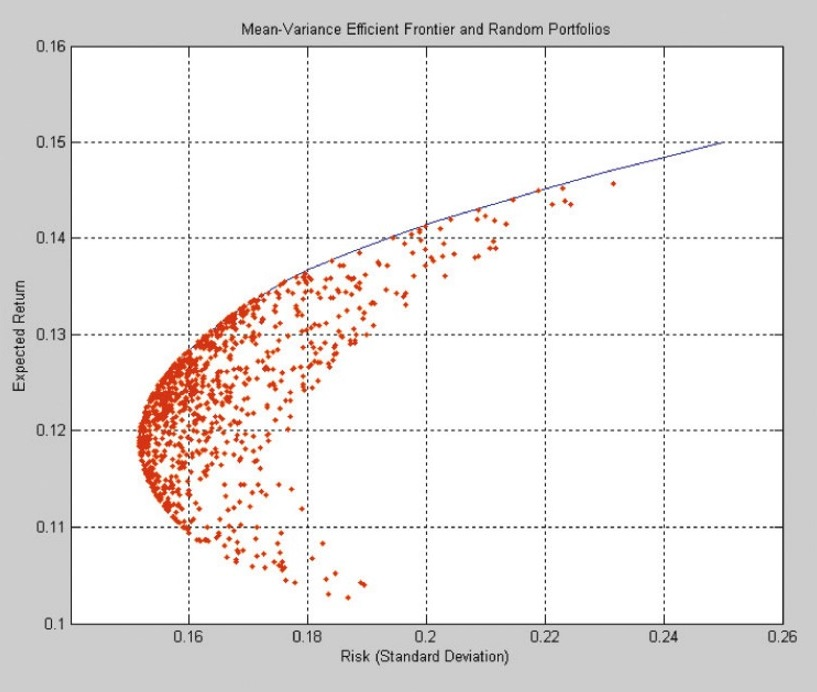
\includegraphics[scale=.5]{risk_management.jpg}
		\end{center}
	\end{addmargin}

	\subsection{Machine Learning}
	Due to lack of historical evidence, it is difficult to train our model to trade using machine learning techniques. This is what initially deterred us from the approach. That said, as a future endeavor, it may be possible to use methods like ``sentiment analysis'' and ``network value to transaction ratio'' to carry out fundamental analysis of cryptocurrencies.
	
	We believe that by incorporating deep machine learning techniques---including pattern recognition---actionable strategies can be uncovered. Instead of relying solely on fundamental analysis to make investing decisions, tools are available that puts the power of machine learning and artificial intelligence in the hands of traders.


\begin{thebibliography}{5}
	\bibitem{1}
	Caldeira, João and Moura, Guilherme V., Selection of a Portfolio of Pairs Based on Cointegration: A Statistical Arbitrage Strategy (January 4, 2013). Available at SSRN: https://ssrn.com/abstract=2196391
	\bibitem{2}
	Avellaneda, M., \& Lee, J. H. 2010. Statistical arbitrage in the US equities market. Quantitative Finance,10, 1–22.

	\bibitem{3}
	Dunis, C. L, Giorgioni, G., Laws, J., \& Rudy, J. 2010. Statistical Arbitrage and High-Frequency Data with an Application to Eurostoxx 50 Equities. CIBEF Working Papers. CIBEF.

	\bibitem{4}
	Robert Richards Chaired Professor of Economics, University of Washington, Chapter 12, Co-integration

	\bibitem{5}
	James V. Burke, Professor of Mathematics, University of Washington, Seattle. Math 408 Section A, Optional Portfolio Optimization Projects, Markowitz Mean-Variance Portfolio Theory Notes
\end{thebibliography}

\end{document}
